\chapter{Introduction}
\markboth{Introduction}{}% To set left/right header
% \localtableofcontents

\section{Context and Objectives}

Robot motion planning is crucial for ensuring efficient and safe robot behavior.
However, robots operating in real-world inevitably face uncertainties, including external disturbances (e.g., wind), model inaccuracies, and state estimation errors.

An effective approach to managing the complexity of robots operating in uncertain real-world environments is the "feedforward/feedback" or "planning/control" paradigm. 
This process involves two main steps:

\begin{enumerate}
  \item Planning Phase (Feedforward): A reference trajectory for the robot states and controls is planned based on available information, such as models of the robot and its environment.
  This step, typically executed offline, incorporates constraints (e.g., collision avoidance, limited actuation) and optimizes metrics like trajectory length or energy efficiency. 
  However, executing this planned trajectory in open-loop often fails in practice due to uncertainties affecting the planned reference.
  \item Control Phase (Feedback): To ensure robust execution, a motion controller is employed to close the loop between the planned and actual motion, compensating for unforeseen effects and uncertainties that were not accounted for during planning.
\end{enumerate}
    
While this sequential approach, which separates planning and control, has proven useful, it exhibits significant limitations:

\begin{itemize}
  \item Modern planners excel at generating feasible and globally optimal paths for high-dimensional systems and complex constraints. 
  However, they typically ignore the role of the runtime feedback controller, leading to two key issues.
  First, the controller must deviate from the planned trajectory to address uncertainties and disturbances, which can quickly compromise feasibility and optimality.
  Then, the planner does not account for the robustness inherently provided by the controller, missing opportunities to generate more robust motion plans.
  \item While many adaptive and robust control schemes (e.g., H-infinity, LPV methods) have been designed to handle uncertainties and disturbances effectively, they are local to the vicinity of a reference trajectory. 
  These methods often fall short when it comes to addressing broader challenges such as feasibility under constraints, global optimality, and performance, which are better managed by global planning approaches.
\end{itemize}
    
To bridge the gap between the two communities, several approaches have been introduced, including more global controllers such as the well-known \gls{mpc}~\cite{cTMPC}. 
In addition, the past decade has seen the rise of so-called 'feedback motion planning'~\cite{cTognon, cContractThMP, cContractThOnlineMP, cMajundarLibrary, cFaSTrack, cRandUpRRT, cRandUP}. 
However, these methods still face challenges related to generalizability, computational efficiency, and their reliance on potentially inaccurate models of the robot/controller pair due to uncertainties in the knowledge of model parameters.

Therefore, this work, based on the 'feedback motion planning' (or 'control-aware motion planning') paradigm shown in Figure~\ref{fig:ca_strat}, leverage the closed-loop sensitivity concept~\cite{cPi,cTh} (an extension of the sensitivity notion that incorporates the controller behavior with respect to parametric uncertainties), in order to create robust control-aware motion planners for a broad class of systems and controllers, while addressing uncertainties in their model representations.

\begin{figure} [htp]
    \centering
    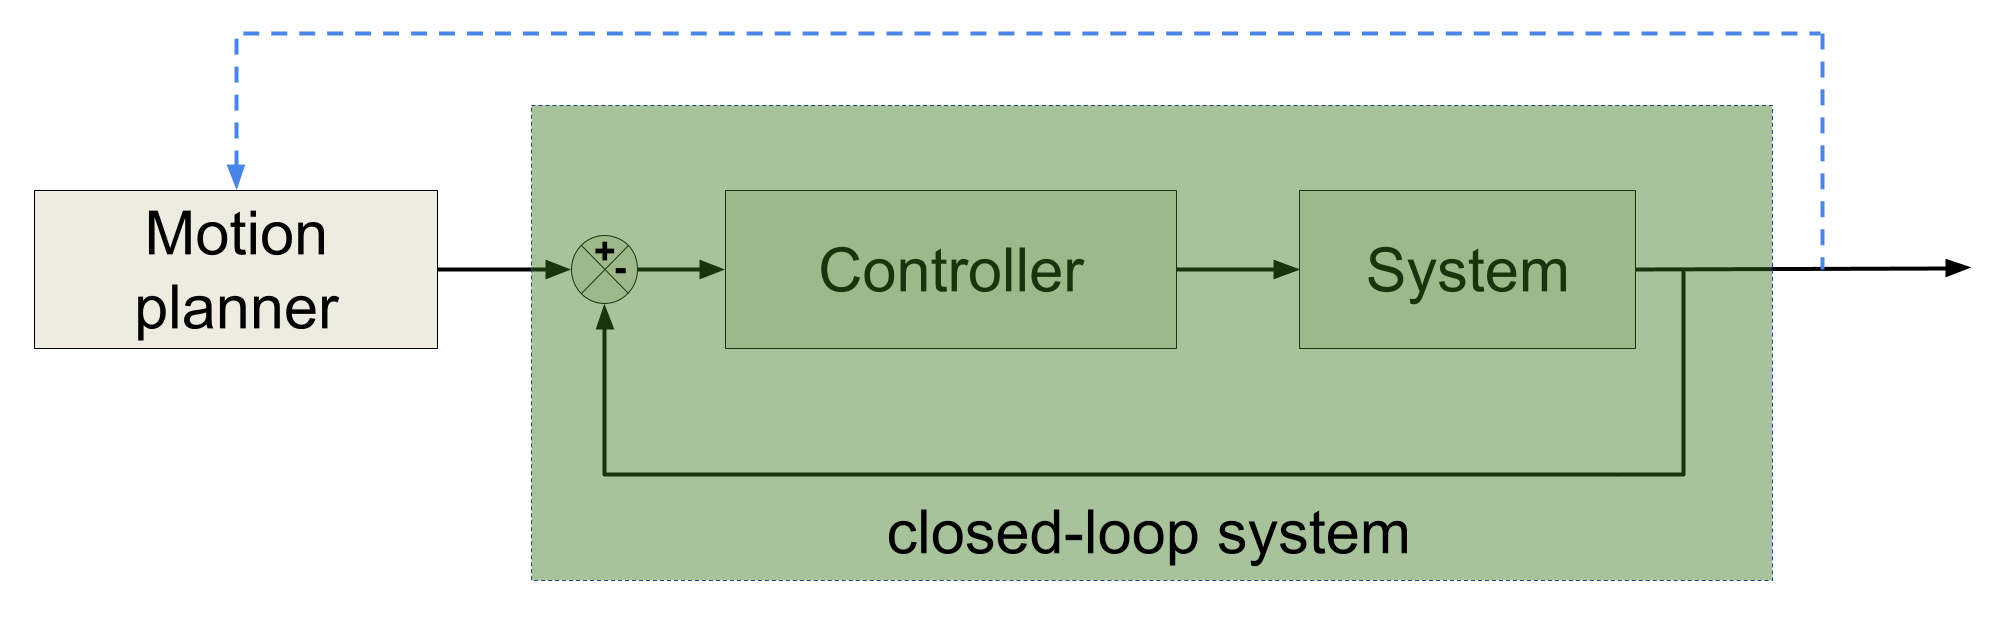
\includegraphics[width=0.9\linewidth]{figures/intro/control-aware.png} 
    \caption{Illustration of the control-aware motion planning strategy.
    It relies on the closed-loop system simulation (green) at the offline motion planning level (gray).}%
    \label{fig:ca_strat}%
  \end{figure}

\section{Thesis Outline}

This manuscript begins with a literature review in Chapter~\ref{chap:related_work}, providing an overview of the current state of the art. 
It initially focuses on decoupled approaches to robust motion planning, starting with path finding methods and progressing to kinodynamic planning paired with robust control strategies.
The review then continues to unified approaches, presenting robust motion planning methods that address uncertainty, as well as control-aware planning techniques. 
The chapter concludes with a focus on unified robust control-aware motion planning approaches, which form the main topic of interest.

Chapter~\ref{chap:models} introduces the \emph{closed-loop sensitivity} concept and present how this concept can be leveraged to derive the so-called uncertainty tubes.
These uncertainty tubes are later employed in this thesis to impose robust constraints on systems while accounting for parametric uncertainties.
Then, this chapter presents the quadrotor and differential drive robot models considered in this thesis, along with their respective controllers and local planning techniques used for generating reference trajectories.

The first contribution of this thesis is then introduced in Chapter~\ref{chap:samp}.
It presents the general method for integrating sensitivity-based uncertainty tubes into sampling-based planners to create various sensitivity-aware motion planner variants.
Furthermore, this chapter emphasizing the generation of sensitivity-optimal trajectories in global context.
Initial simulation results, using the models introduced in Chapter~\ref{chap:models}, highlight that computing uncertainty tubes become a bottleneck for sampling-based methods.
To address this, a more efficient variant is proposed, leveraging a lazy collision-checking approach to reduce the frequency of uncertainty tube computations.

Chapter~\ref{chap:NN} introduces the second major contribution of this thesis, which leverages the structural similarities between ordinary differential equations and recurrent neural network cells to accelerate the computation of sensitivity-based uncertainty tubes. 
A dataset generation method, based on sampling-based principle, is proposed and applied to the models discussed in Chapter~\ref{chap:models}. 
The method achieves an optimal balance between inference time and accuracy, making it highly effective for motion planning and showcasing the efficiency of the approach.

Chapter~\ref{chap:sampNN} aims to integrate the sensitivity-aware motion planning variants introduced in Chapter~\ref{chap:samp} with the deep learning approach detailed in Chapter~\ref{chap:NN}, resulting in a more efficient version of the sensitivity-aware motion planner variants.
Furthermore, while the previous chapters solely focus on generating robust and sensitivity-optimized trajectories, this chapter emphasizes the generation of task-specific accurate trajectories.
The effectiveness of this contribution is finally demonstrated through experimental validation on two challenging scenarios requiring high robustness and accuracy.

Finally, Chapter~\ref{chap:concl} presents an overall conclusion that summarizes the contributions of this thesis along with their limitations.
Additionally, several perspectives are outlined to improve the generalizability of the proposed approach.

\section{Thesis Contributions}

The work conducted throughout this thesis led to the following publications in international peer-reviewed conferences and letters. 

~\cite{cSAMP} Wasiela, S., Giordano, P. R., Cortés, J., and Simeon, T. (2023, May). "A sensitivity-aware motion planner (samp) to generate intrinsically-robust trajectories." In IEEE International Conference on Robotics and Automation (ICRA) (pp. 12707-12713).

~\cite{cECAI}: Wasiela, S., Bouhsain, S. A., Cognetti, M., Cortés, J., and Simeon, T. (2024, October). "Learned Uncertainty Tubes via Recurrent Neural Networks for Planning Robust Robot Motions." In 27th European Conference on Artificial Intelligence (ECAI) (pp. 4385-4392).

~\cite{cRAL}: Wasiela, S., Cognetti, M., Giordano, P. R., Cortés, J., and Simeon, T. (2024). "Robust Motion Planning with Accuracy Optimization based on Learned Sensitivity Metrics." In IEEE Robotics and Automation Letters (RA-L).

Belvedere, T., Afifi, A., Wasiela, S., and Pupa, A. (2025, March). "Planning under Uncertainties with Closed-Loop Sensitivity: Recent Results and Perspectives." In European Robotics Forum (ERF).

Furthermore, all implementations presented and used in this thesis are available at: \href{https://gitlab.laas.fr/CAMP}{https://gitlab.laas.fr/CAMP}.